\providecommand{\main}{../../../..}
\documentclass[\main/dresen_thesis.tex]{subfiles}
\renewcommand{\thisPath}{\main/chapters/theoreticalBackground/ferrites/maghemite}
\begin{document}

  \begin{figure}[htbp]
    \centering
    % 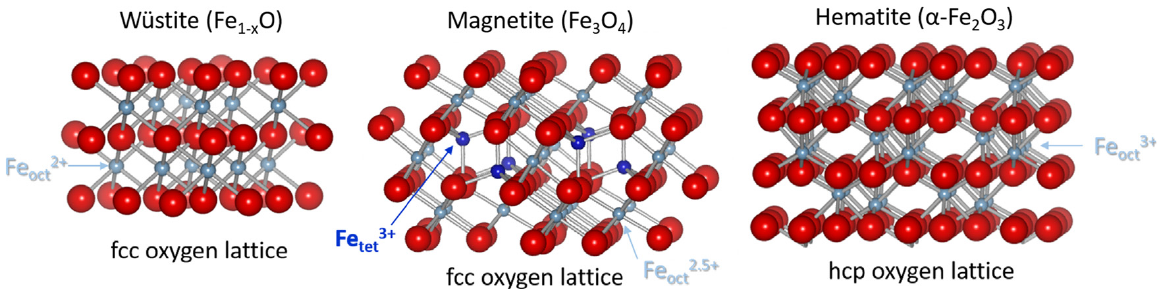
\includegraphics[width=\textwidth]{ferrites_iron_oxides_structures}
    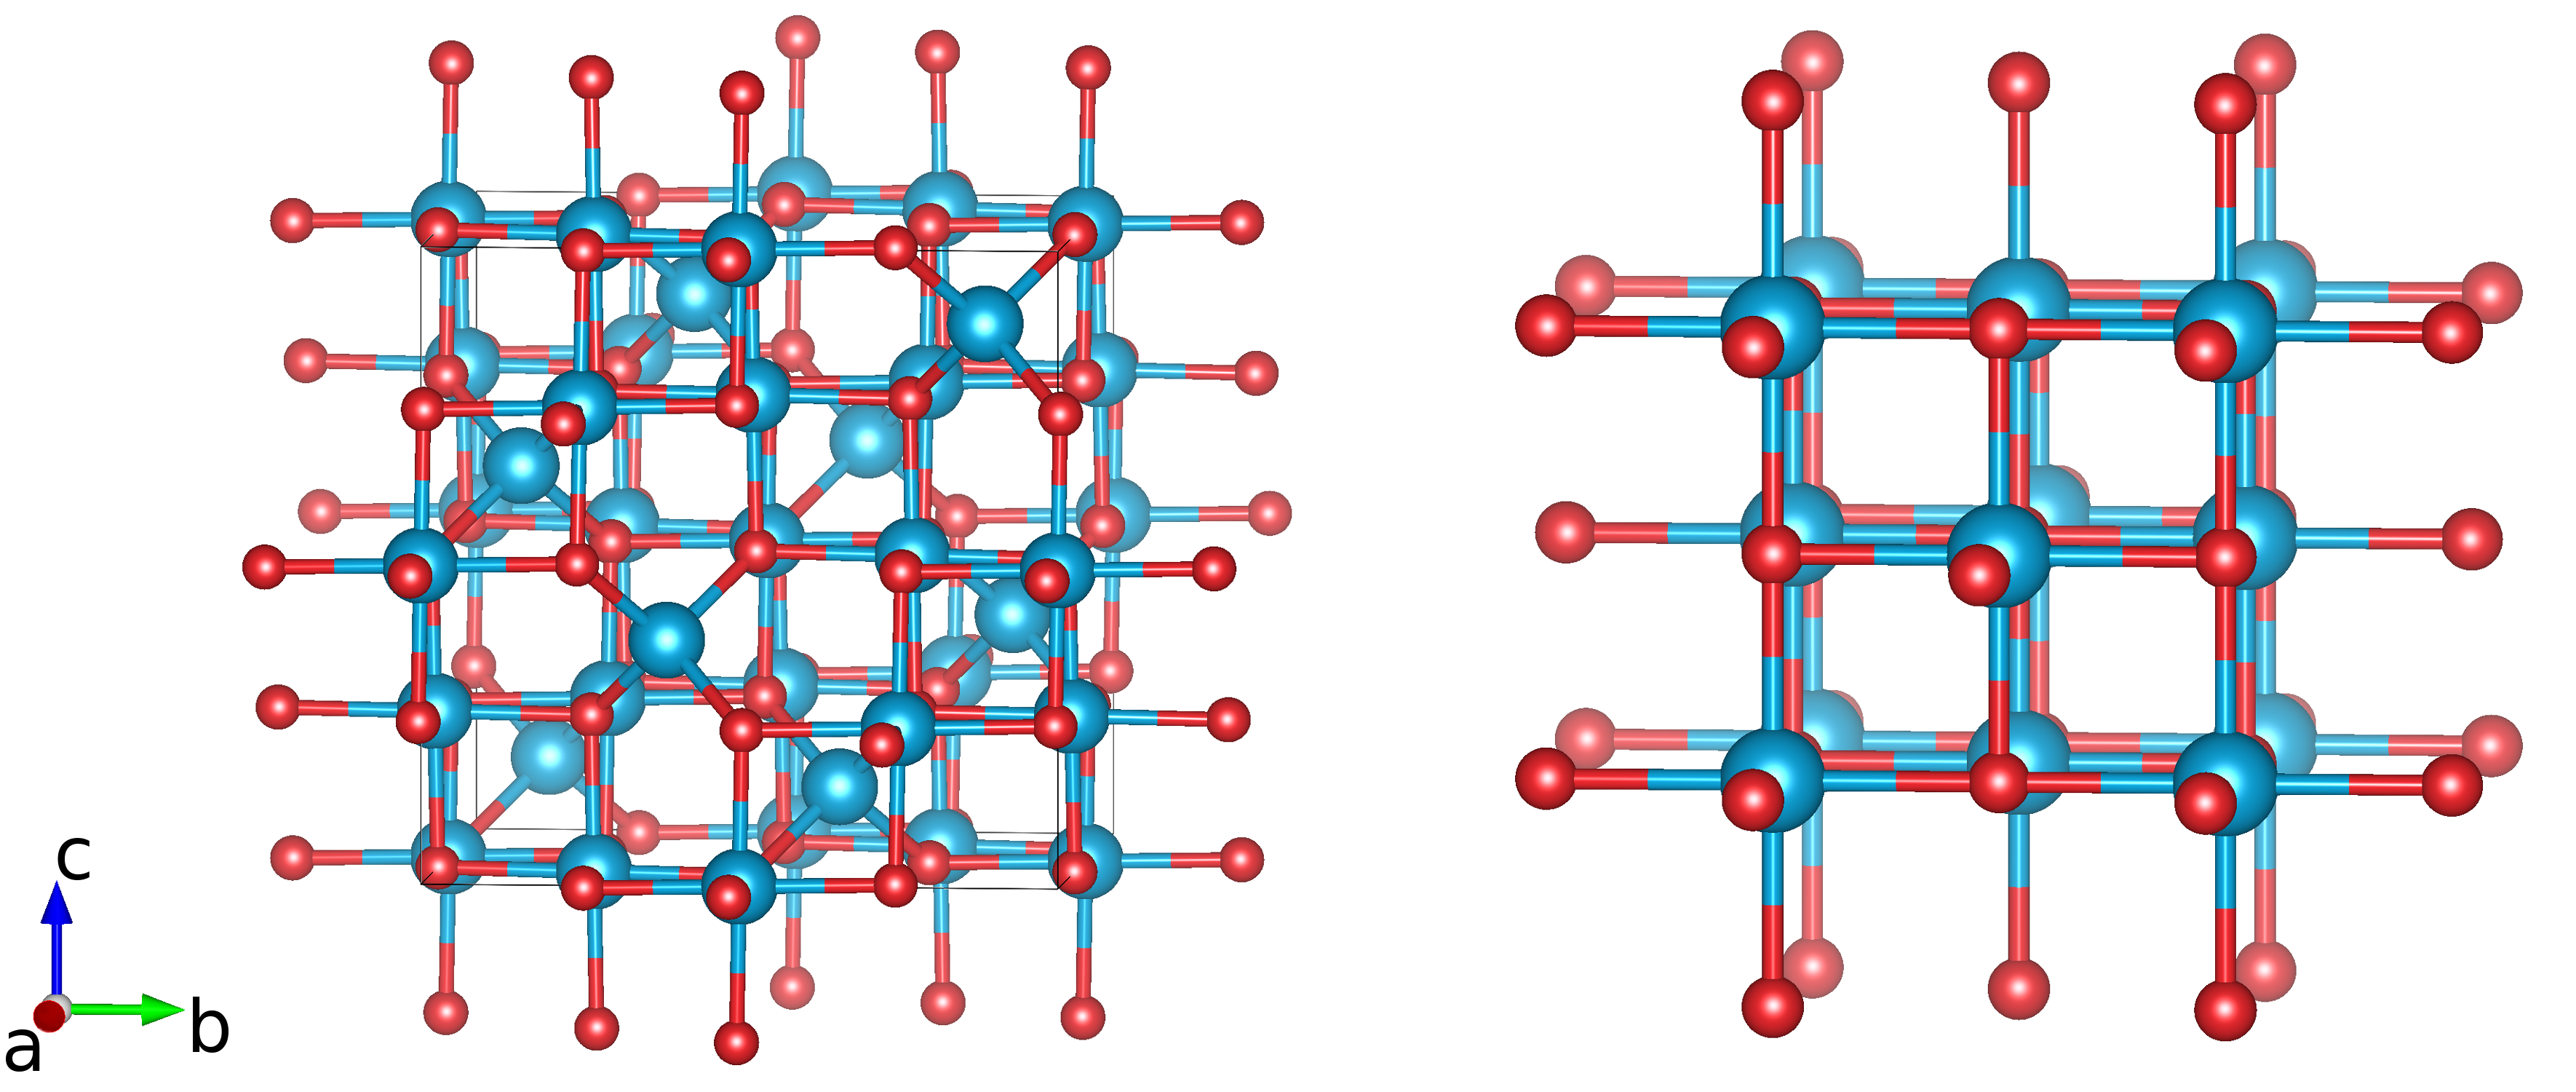
\includegraphics{theoreticalBackground_spinels_MagnetiteWustite}
    \caption{\label{fig:theoreticalBackground:ferrites:ironOxides}Iron oxide structures of magnetite (left) and w\"ustite (right). The red spheres represent the close packed \ch{O^{2-}} lattice and the iron cations occupy either the tetrahedral or octahedral interstices, where different configurations with different oxidation states result in the various compounds. The visualization were produced with the VESTA software \cite{Momma_2011_Vesta} using the crystallographic information files 9007706 \cite{Fleet_1984_Thest} for magnetite and 9008636 for w\"ustite \cite{Wyckoff_1963_Secon}.}
  \end{figure}
  When both $\ch{Fe^{2+}}$ and $\ch{Fe^{3+}}$ are present upon crystal formation, magnetite (\ch{Fe3O4}) forms as the stable phase with the structure of an inverse spinel in the space group $Fd\bar{3}m$ and a lattice constant of $a \eq 8.396 \unit{\angstrom}$ \cite{Cornell_2003_Their}.
  It's unit cell is depicted in \reffig{fig:theoreticalBackground:ferrites:ironOxides}.
  The inverse spinel structure of a compound \ch{AB2O4} is commonly noted as \ch{(B)[AB]O4}, where the round bracket notes the atoms in the tetrahedral and the square bracket the atoms in the octahedral position \cite{Sickafus_1999_Struc}.
  Magnetite is noted by (\ch{Fe^{3+}})[\ch{Fe^{2+}Fe^{3+}}]$\ch{O4}$, meaning in a unit cell with $32$ oxygen anions, the A-sublattice of eight tetrahedral positions is occupied by $\ch{Fe^{3+}_A}$ and the B-sublattice of 16 octahedral sites is occupied half by $\ch{Fe^{2+}_B}$ and half by $\ch{Fe^{3+}_B}$.
  From M\"ossbauer experiments it is observed that the iron cations on the B-sublattice can be considered in a mixed valence state $\ch{Fe^{2.5+}_B}$ resulting from a electron hopping mechanism between $\ch{Fe^{2+}_B}$ and $\ch{Fe^{3+}_B}$ \cite{Cornell_2003_Their}.
  The spins of the iron cations interact via a superexchange interaction antiferromagnetically for the A-A and A-B bonds and ferromagnetic for the B-B bonds \cite{Mazozuluaga_2007_Surfa}, which results in the ferrimagnetic state of magnetite.
  The saturation magnetization of bulk magnetite is in the order of $475 - 517 \unit{kA m^{-1}}$ \cite{Cornell_2003_Their, Handley_2000_Moder}.
  At room temperature, bulk magnetite has a cubic magnetocrystalline anisotropy with [111] and [100] being the easy and hard axis respectively, with a first-order magnetocrystalline constant of $K_1 \eq -1.35 \cdot 10^{4} \unit{J\, m^{-3}}$ \cite{Goya_2003_Stati}.
  At temperatures below the Verwey temperature $T_V \eq 120 \unit{K}$ \cite{Bickford_1957_Magne}, the cubic structure transitions to a triclinic structure, which yields a change to uniaxial anisotropy with near [001] as easy axis \cite{Medrano_1999_Domai}.

  When magnetite is oxidized at low temperatures, maghemite ($\gamma-\ch{Fe2O3}$) forms which is a defective inverse spinel only composed of $\ch{Fe^{3+}}$ and additional vacancies in the octahedral sites to ensure charge neutrality, noted by $(\ch{Fe^{3+}})[\ch{Fe^{3+}}_{5/3}\square_{1/3}]\ch{O4}$.
  The lattice constant of bulk maghemite is found in literature to be $a \eq 8.340 \unit{\angstrom}$ \cite{Cornell_2003_Their}.
  The magnetism of maghemite is analogue to magnetite ferrimagnetic at room temperature, where the trivalent cations on the tetrahedral and octahedral sites are antiferromagnetically coupled by a super-exchange interaction mediated by the oxygen anions.
  The bulk saturation magnetization at $300 \unit{K}$ is found in literature to be in the range of $290 - 390 \unit{kA m^{-1}}$ and the cubic magnetocrystalline anisotropy constant is reported in the range of $K_1 \eq -(1.7 \ldots 10) \cdot 10^{4} \unit{J \, m^{-3}}$ \cite{Cornell_2003_Their}
  The coercive field of both single-domain magnetite and maghemite resulting from the magnetocrystalline anisotropy is in the order of $30 \unit{mT}$ and the critical diameter for the transition from single domain to pseudo-single domain is for both phases in the order of $30 - 100 \unit{nm}$ \cite{Cornell_2003_Their}.

  It is noteworthy that maghemite is a metastable iron oxide state.
  For fully oxidized iron upon exposure to elevated temperatures, the compound transitions to hematite with the oxygen anions on a \textit{hcp} lattice and all $\ch{Fe^{3+}}$ on octahedral sites.
  Hematite is only weakly ferromagnetic at room temperature and antiferromagnetic below $T \eq 260 \unit{K}$ \cite{Cornell_2003_Their}.

  On the other side of the spectrum, in a strongly reducing environment with only $\ch{Fe^{2+}}$ present, w\"ustite (\ch{Fe_{1-x}O}) is the stable phase, which crystallizes typically in a defective rocksalt structure where oxygen forms an \textit{fcc} lattice and deficient \ch{Fe^{2+}} occupies the octahedral sites.
  The unit cell is depicted also in \reffig{fig:theoreticalBackground:ferrites:ironOxides}.
  The lattice constant of w\"ustite ranges from $4.28 - 4.31 \unit{\angstrom}$ depending on the vacancy content \cite{Cornell_2003_Their}.
  W\"ustite is paramagnetic at room temperature with a room temperature susceptibility of $\mu_0 \chi \eq 7230 \cdot 10^{-6}$ \cite{Lide_2004_Handb} and antiferromagnetic at temperatures below $T_N \approx 203 K$ \cite{Cornell_2003_Their}.

\end{document}